\chapter{Background}\label{chap:background}
The title of this thesis is \textit{\thesisTitle}.
It brings together the domains of Process Science (hence Events), Predictive Modeling and Deep Learning.
This chapter gives insights into these topics that will be used and needed throughout the thesis.
This work can be attributed to the domain of Predictive Process Monitoring, which will also be introduced.

\section{Process Science And Process Monitoring}
Process Science, as loosely defined by van der Aalst \cite{Aalst2016}, refers to the \textit{broader discipline that combines knowledge from information technology and knowledge from management sciences to improve and run operational processes}. This means that approaches in this domain tend to be model-driven, like Six Sigma or Kaizen.

Central to process science is Business Process Management (BPM) and process models.
These models have traditionally been modeled in a very rigid manner, for example using the Business Process Modeling Notation (BPMN) \cite{bpmn2.0}.
With the help of workflow management systems (WFMS), it became possible to embed and enforce structured processes in an organization.
\todo[inline]{taxonomy for variability in processes}

While model-driven, WFMS permitted some flexibility in processes and, most importantly for this thesis, logged execution traces of running process instances. With the increasing amount of logs, it became obvious that rigid models were not suited equally well for all types of processes. Especially in the insurance and health-care sector, each instance of a process tended to be very different from the next. This led to the notion of a case, and that its course strongly depended on the information contained inside it. 

\subsection{Adaptive Case Management}
In settings in which it is common to employ BPM, such as assembly line productions, there is little heterogeneity. As the latter increases, BPMN and other business process modeling notations result in complex and hardly understandable models and thus fail their purpose. As previously mentioned, such cases tend to occur in domains where the trajectory is highly dependant on information specific to a case.

The fact that this type of process is data-driven, led to the creation of the concept of a case folder - a directory central to a case, describing its current state. In contrast to BPM, the formalization of ACM and the subsequent creation of modeling languages has only just begun. Notable efforts include the Case Management Modeling Notation \cite{web:cmmn} as well as the Chimera approach \cite{hewelt2016}.



\subsection{Predictive Process Monitoring}
This enabled Process Mining and data-driven process optimization through the discovery of bottlenecks.
As Process Mining makes use of data processing analysis techniques common in the area of data science, it is common to understand is as a bridge between the two domains, as shown in \autoref{fig:process-data-science}.
\begin{figure}
    \centering
    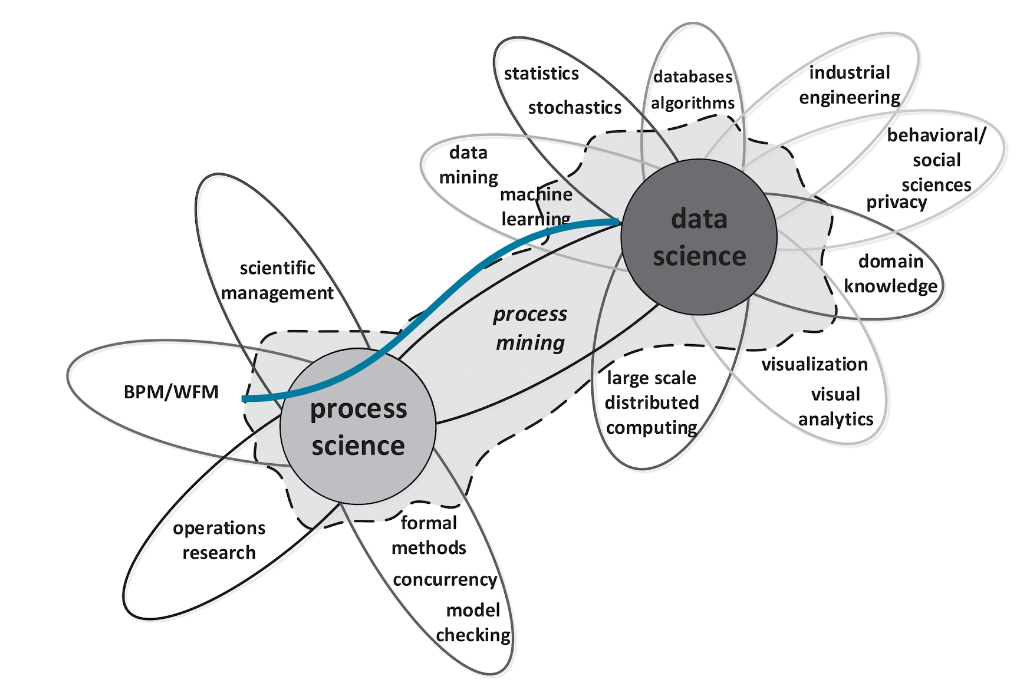
\includegraphics[width=\textwidth]{gfx/process-data-science.png}
    \caption{Caption}
    \label{fig:process-data-science}
\end{figure}

Somewhere between Process Science and Data Science
Process science revolves around managing and optimizing structured procedures, while the broad area of data science covers data mining, algorithmic analysis and predictive analytics. 
Bridging the gap between the two fields is process mining \cite[p.18]{Aalst16}.
It covers the three steps of model discovery, conformance checking and model enhancement \cite{Aalst16}.

These three steps are focused on offline data.
If one would like to avoid a certain process outcome  or e.g. an SLA violation, a guess at future developments requires resorting to online data analysis.
At this step, techniques from the domain of predictive analytics can be employed\footnote{More detail from Marlon Dumas on how these topics fit together: \url{https://www.youtube.com/watch?v=hMQolsRT0K0}}.

Predictive analytics brings together a variety of statistical techniques like data mining, predictive modelling, and machine learning in order to make predictions about future events throught the use of historical data.
In the domain of business processes, statistical or machine learning models are trained with historical process execution logs and \textit{target} a specific piece of data that should be predicted.
This application is called predictive process monitoring and allows answering questions such as \textit{Given the current state of things, will I still meet my SLA?} or \textit{Given the current case state, how long is this case still going to take?}.
The answers to such questions can give case managers the opportunity to intervene if a case takes an unwanted course or might fail to meet KPI requirements.


\begin{figure}
	\centering
	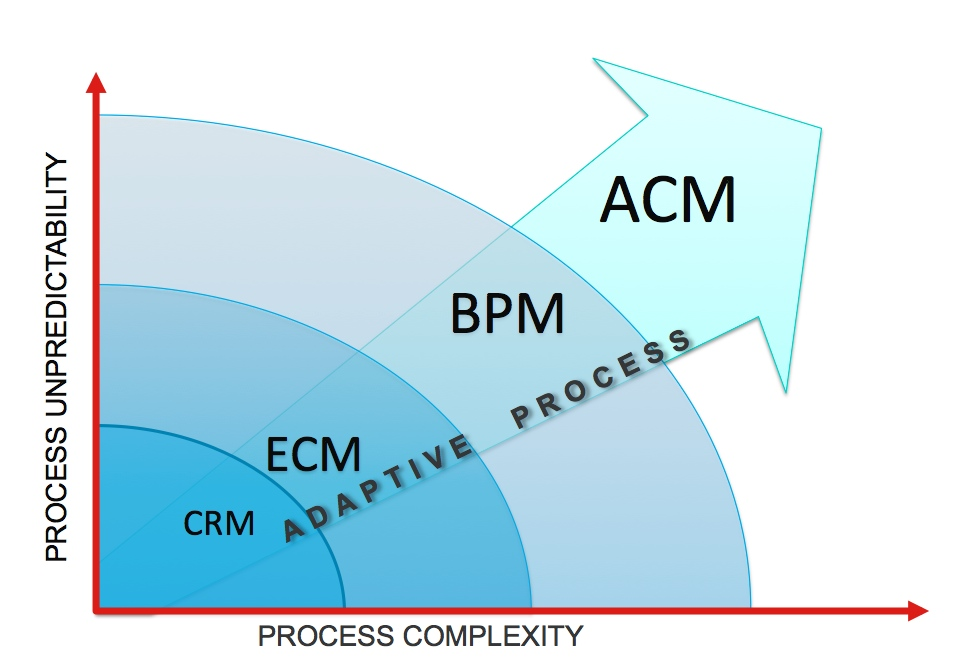
\includegraphics[width=\textwidth]{gfx/acm-reasoning}
	\caption{https://acmisis.wordpress.com/what-is-adaptive-case-management-acm/}
	\label{fig:why-acm}
\end{figure}

\section{Predictive Modeling}
\subsection{Subsequence Mining}

\section{Predictive Modeling}
\subsection{Knowledge Discovery in Databases}
\begin{figure}
	\centering
	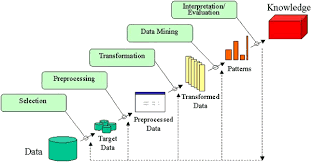
\includegraphics[width=\textwidth]{gfx/kdd_process}
	\caption{The process for \textit{Knowledge Discovery in Databases}}
	\label{fig:kdd_process}
\end{figure}
Predictive analytics is a lot about model training, and the rough outline of necessary steps necessary to train a model is listed here:
\begin{enumerate}
	\item Determine the \textit{target} variable, it is the variable that is supposed to be predicted
	\item Preprocess the dataset. This can mean introducing one-hot encodings, normalized values, but also basic data quality assurance such as null value elimination. Feature engineering can also happen at this step.
	\item Partition the dataset into two parts. One part is set aside for model performance verification, as there the actual target variable value is known. This is commonly referred to as the \textit{test set}, while the remainder is called the \textit{training set}.
	\item Train the model on the training set. Models are trained multiple times with different hyper-parameters to find the optimum configuration with respect to prediction accuracy on the test set. Hyper-parameters are model-specific values such as cutoff-thresholds that have impact on model performance.
\end{enumerate}

\subsection{Language Modeling}
\subsubsection{Sequence-to-Sequence prediction}
\subsubsection{Sequence-to-word prediction}

\subsection{Popular feature engineering techniques}
\subsubsection{Sliding Window}
\subsubsection{N-gram}
\subsubsection{Bag-Of-Words}
\subsubsection{Learned features, word2vec}
Strictly piecewise\\
subsequences, embedding
PrefixSpan

\subsection{Neural networks}
\subsubsection{RNN}
\subsubsection{LSTM memory}